\chapter{Designing and Fabricating the Enclosure: 3D Modeling and Printing}
\label{cap:3dModelingAndPrinting}

Designing and fabricating enclosures for electronic devices involves choosing the most suitable 
fabrication method. Various methods exist, ranging from traditional machining and molding 
techniques to more modern additive manufacturing processes. Among these, 3D printing has become 
one of the most accessible and cost-effective methods, especially for small-scale productions and 
prototypes.

Unlike traditional manufacturing processes that may require expensive tooling and setups, 3D 
printing has minimal upfront costs to get started. This makes it particularly attractive for rapid 
prototyping and custom design iterations. The ability to create complex geometries and designs 
with relative ease also contributes to its popularity in the field of electronics.

In this chapter, the process of designing and fabricating the enclosure for the employee time 
tracking device using 3D modeling and printing techniques is explored. The chapter discusses the 
design considerations, the software tools used for modeling, and the intricacies of the 3D 
printing process. Additionally, it examines the challenges encountered and the solutions 
implemented during this phase.


\section{3D Modeling}

3D modeling plays a crucial role in the design and fabrication of the enclosure for the employee 
time tracking device. It enables precise visualization and customization of the physical form of 
the device, accommodating its electronic components and ensuring functional and aesthetic 
requirements are met. This section explores the process of 3D modeling, detailing the software 
tools utilized, the design considerations, and the iterative development of the enclosure design. 

\subsection{An Iterative Process}

The first step in designing the enclosure was to decide on a general shape. The primary objective 
was to create an enclosure that was as compact as possible while remaining visually appealing and 
functional. A rectangular shape was chosen, with the layout designed to maximize usability and 
accessibility. The top third of the enclosure would be occupied by the screen, providing a clear 
display for users, while the lower two-thirds would house the NFC reader, the Raspberry Pi, and 
the PCB. This can be seen in Figure \ref{fig:enclosure_front}.

\begin{figure}[h]
	\centering
	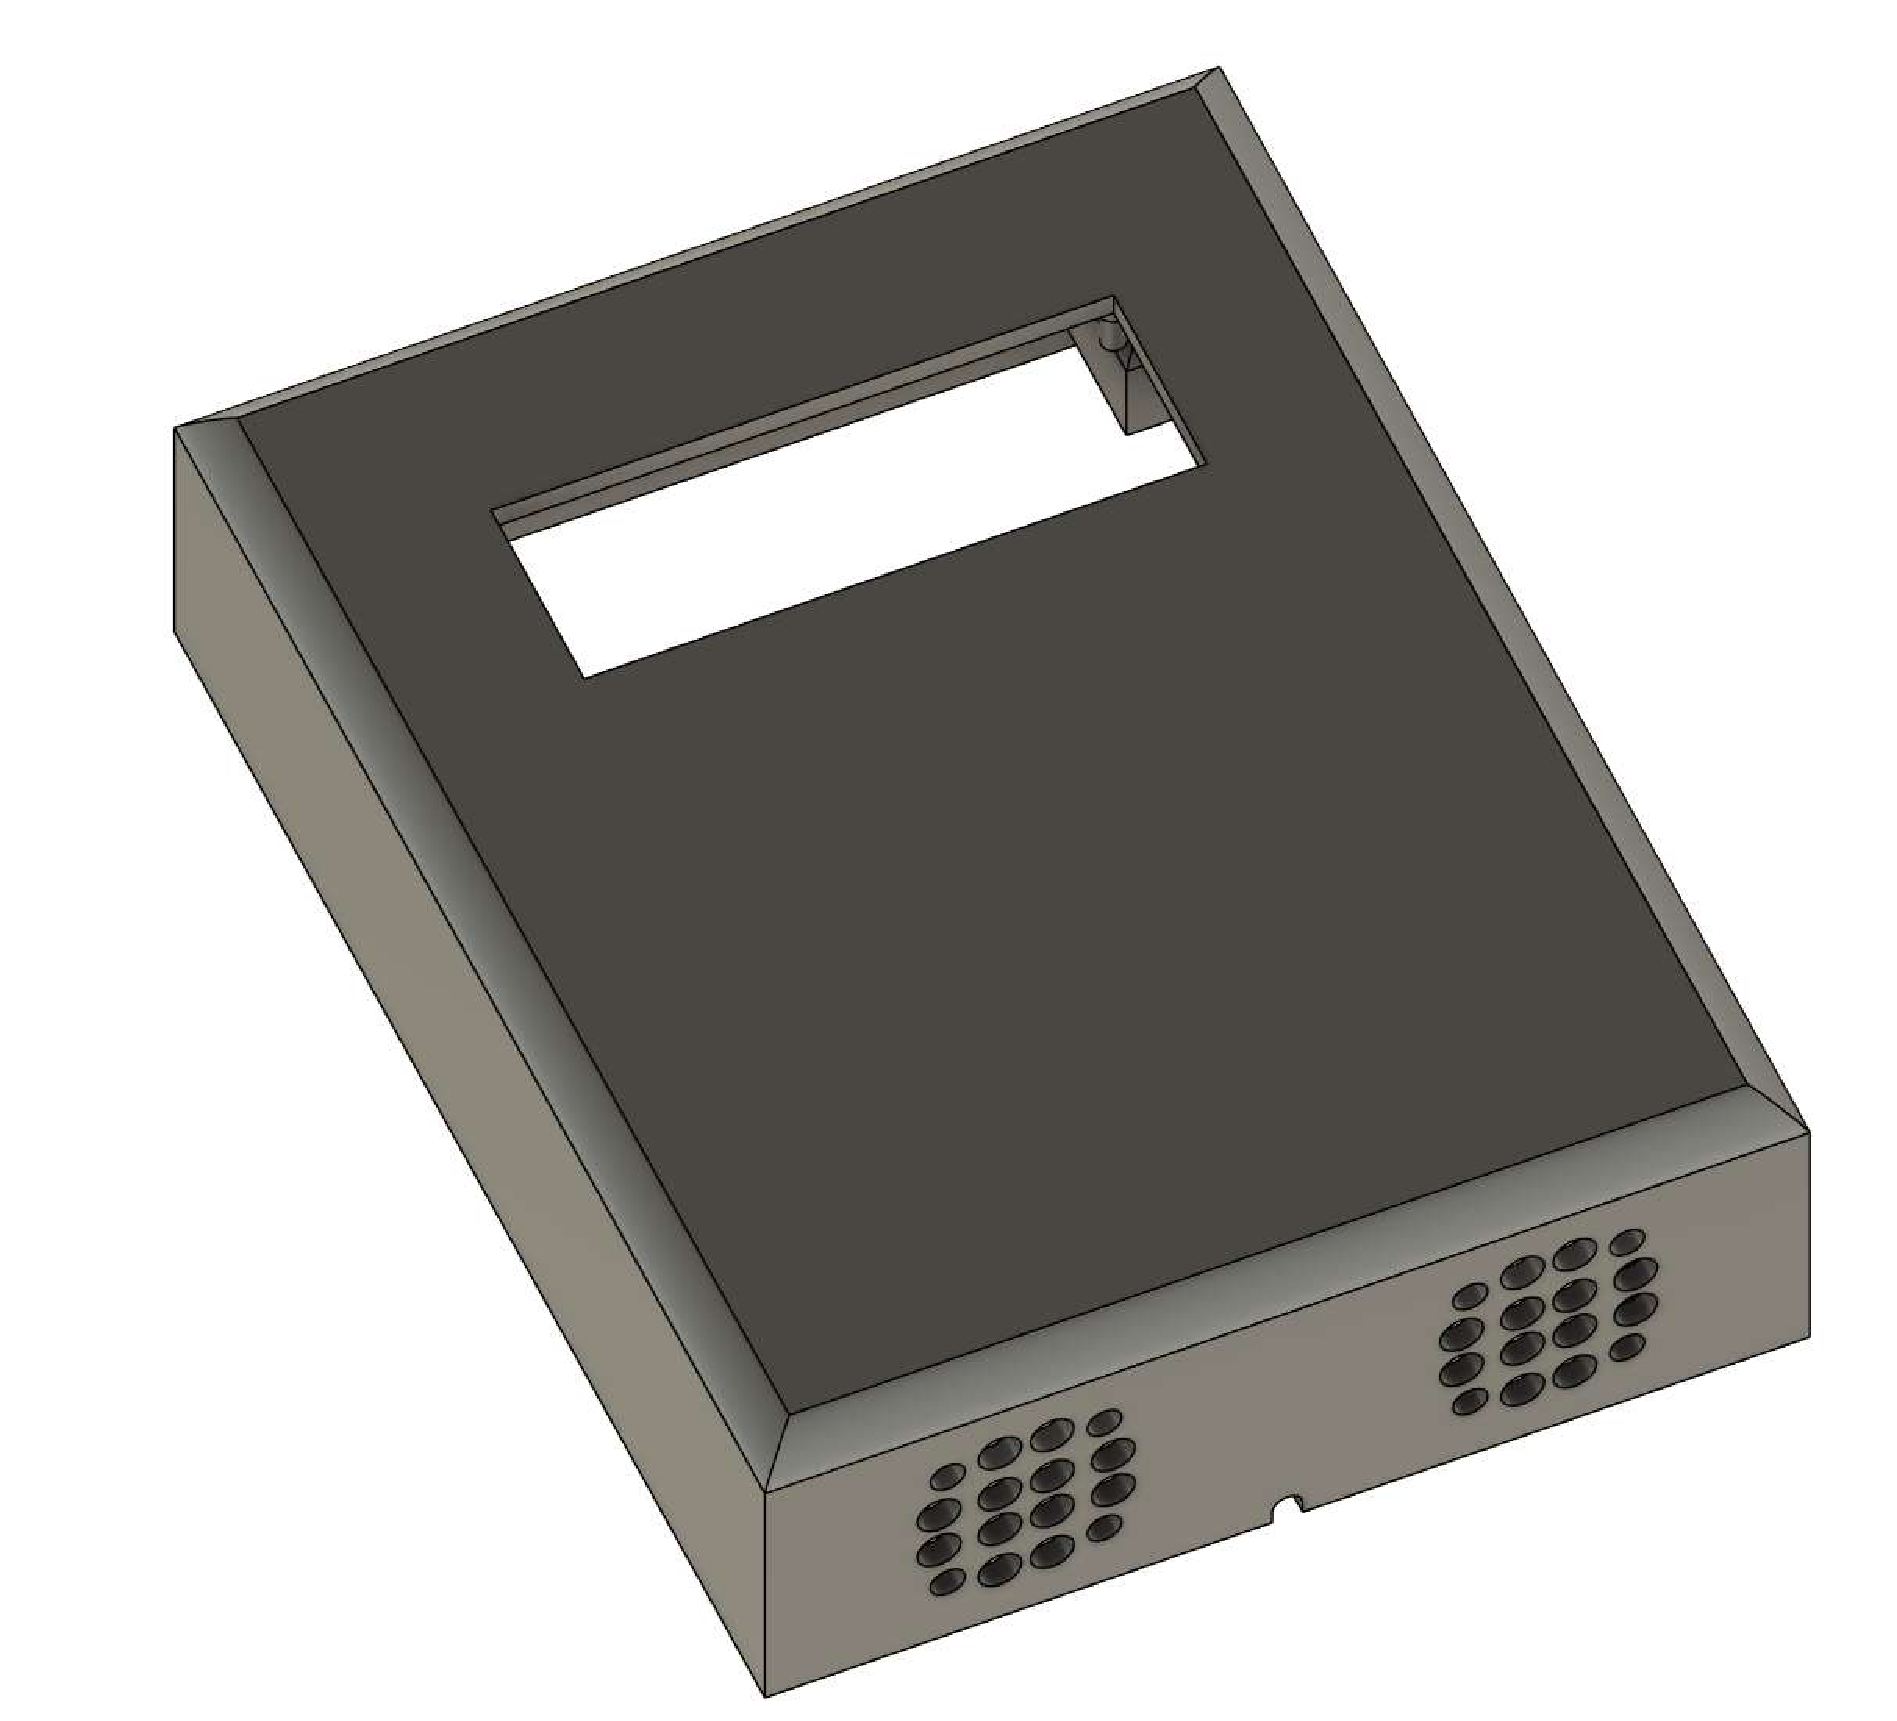
\includegraphics[width = .5\textwidth]{Imagenes/Vectorial/enclosure_front.pdf}
	\caption{Enclosure view from the top}
	\label{fig:enclosure_front}
\end{figure}

To bring this design to life, Fusion 360\footnote{Fusion 360's Website: 
\url{https://www.autodesk.es/products/fusion-360/overview}}, developed by Autodesk, was selected 
as the modeling software. Fusion 360 is an industry-leading solution renowned for its versatility 
and widespread use in 3D modeling for various applications, including product design and 
engineering.

Ensuring the secure attachment of the components to the enclosure was critical. The mounting holes 
present in the NFC reader's board, the display, and the PCB were utilized for this purpose. 
Precise measurements were taken using a caliper to model the studs accurately in Fusion 360. These 
measurements ensured that the components would fit snugly and securely within the enclosure.
Considering that the device had to be as compact as possible, the NFC reader and the PCB were 
stacked one on top of the other, making for an extremely compact design.

In the first design iteration, threaded studs were incorporated into the model. Corresponding nuts 
were also designed to secure these studs. Although the threads functioned as intended, they proved 
to be problematic. The studs, being less than 3 millimeters in diameter, were too fragile. They 
tended to break easily if the enclosure was dropped, and the threads often sheared off, making it 
difficult to release the components without breaking the studs. This initial challenge highlighted 
the need for a more robust solution in subsequent design iterations.

It is also worth noting that even with the studs at the full 3-millimeter diameter, they remained 
fragile and prone to breaking when dropped. This issue manifested during testing, necessitating a 
more robust solution.

Consequently, walls were added to surround the NFC board and the PCB. These walls featured extra 
support at their lower parts but lacked support near the top. This design allowed the walls to 
act like springs during a drop, absorbing impact and preventing the boards from breaking the 
studs. This solution proved highly effective and was incorporated into the final design. This 
can be seen in Figure \ref{fig:enclosure_walls}.

\begin{figure}[h]
	\centering
	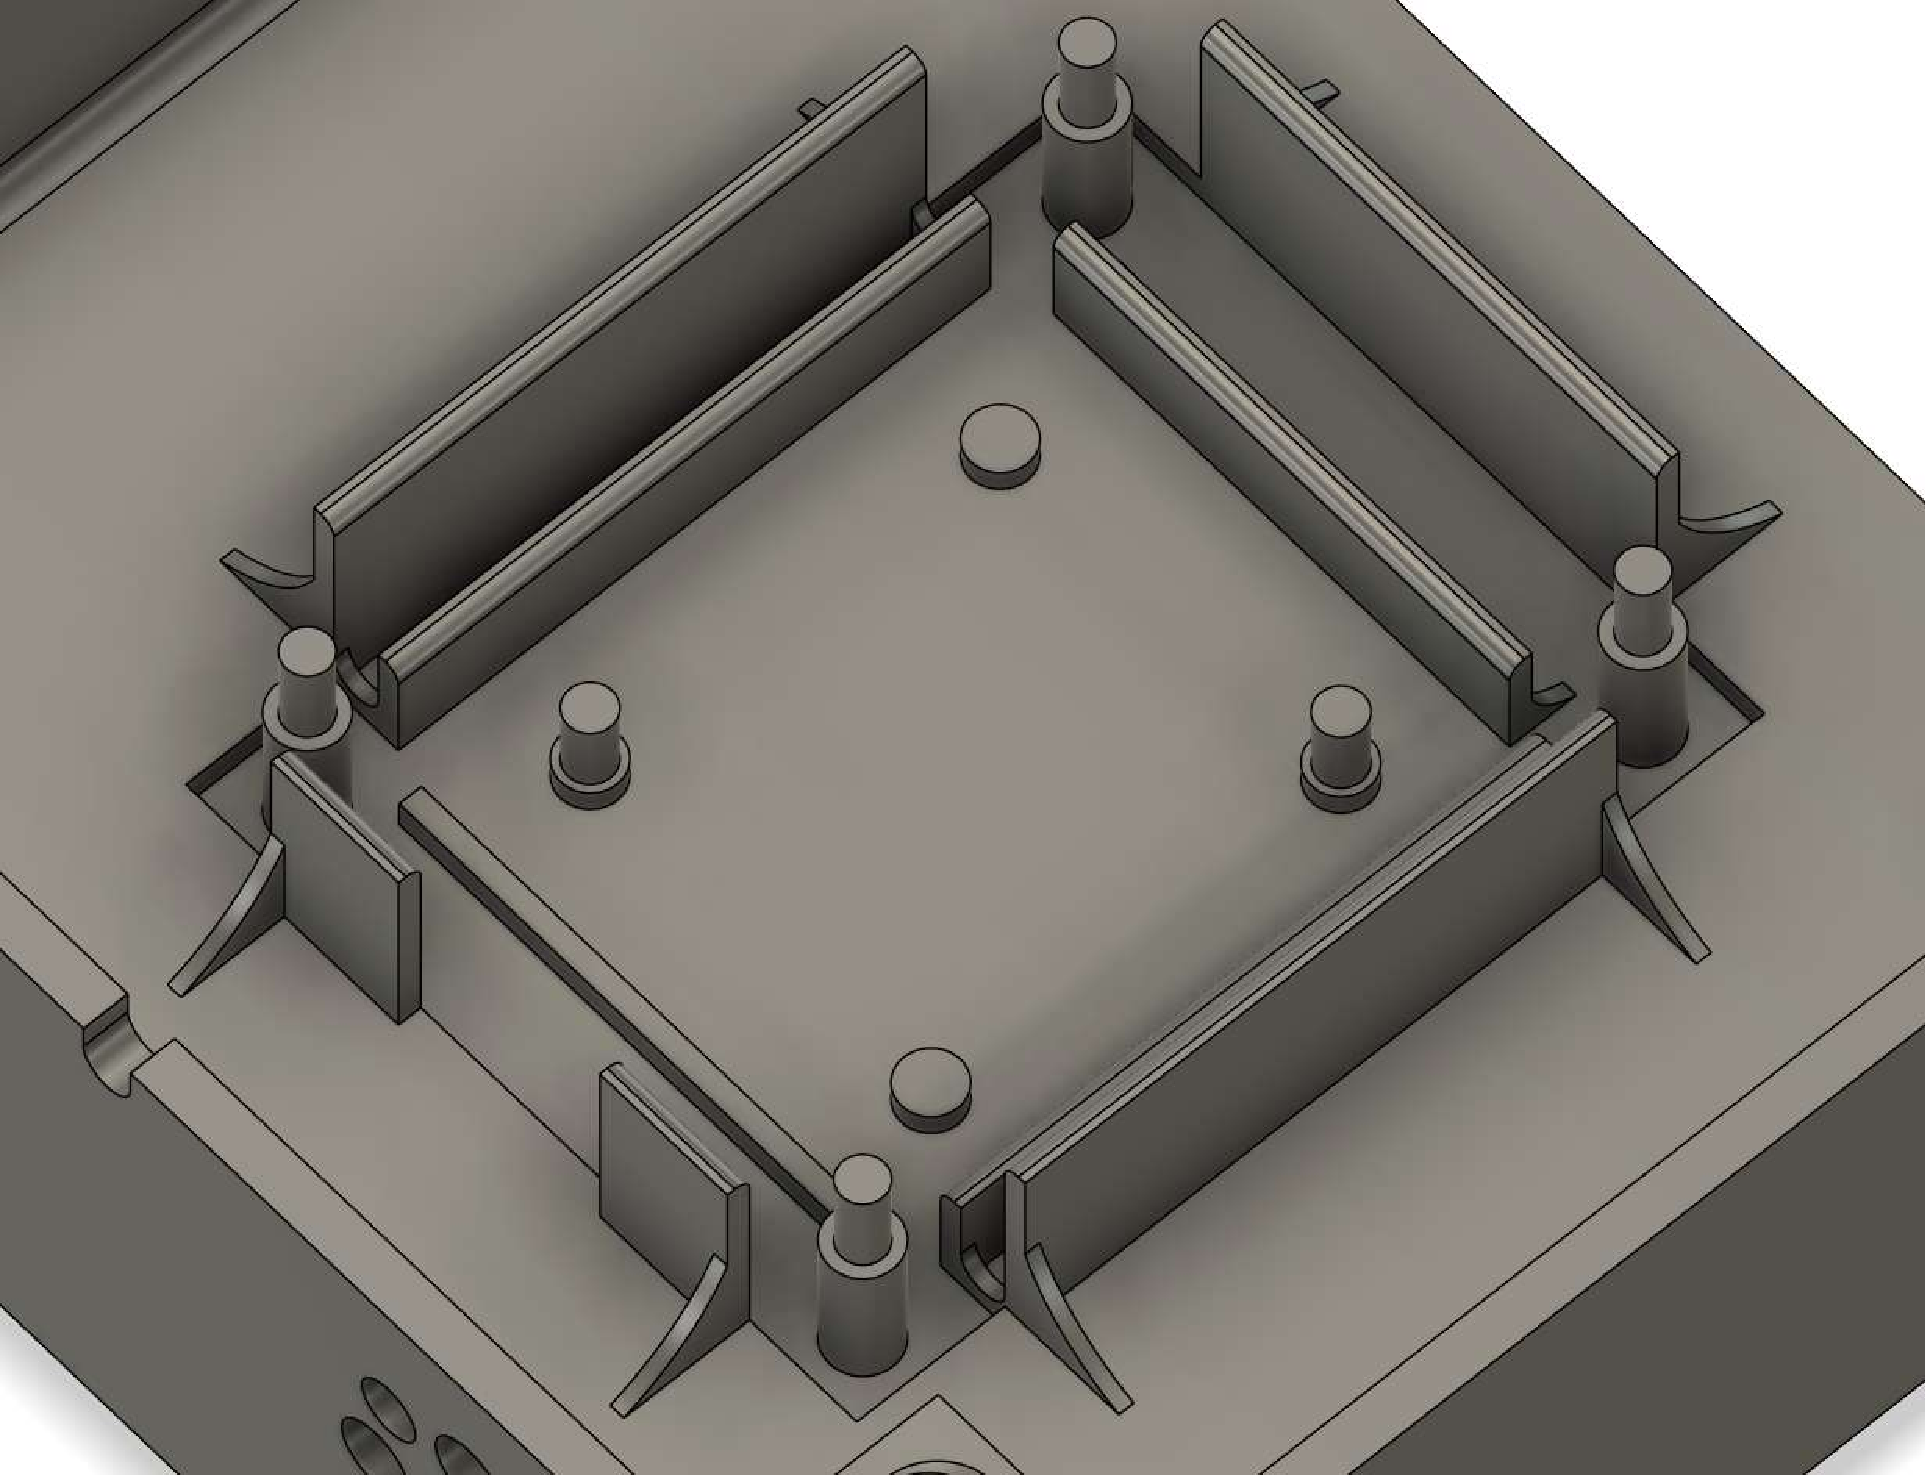
\includegraphics[width = .5\textwidth]{Imagenes/Vectorial/enclosure_walls.pdf}
	\caption{Enclosure's ``walls''}
	\label{fig:enclosure_walls}
\end{figure}

However, a new issue arose with the removal of the threaded studs: there was no way to prevent the 
components from moving up and down or shooting out of their positions. The solution came in the 
form of a backplate that would be screwed on the back of the enclosure. The height of the 
device was designed so that the backplate would press the Raspberry Pi Pico against the PCB and 
the base of the studs, preventing any movement. For the LCD display, four hollow cylinders were 
designed to press against the back of the LCD, ensuring it remained securely in place. This can be 
seen in Figure \ref{fig:backplate_front}. Notably, the LCD display did not require additional 
walls for support, as it was already held in place by protruding outside the enclosure. In this 
way, the final design successfully addressed the issues of component stability and impact 
resistance, ensuring a robust and reliable enclosure for the device.

\begin{figure}[h]
    \centering
    \begin{minipage}[b]{0.49\textwidth}
        \centering
        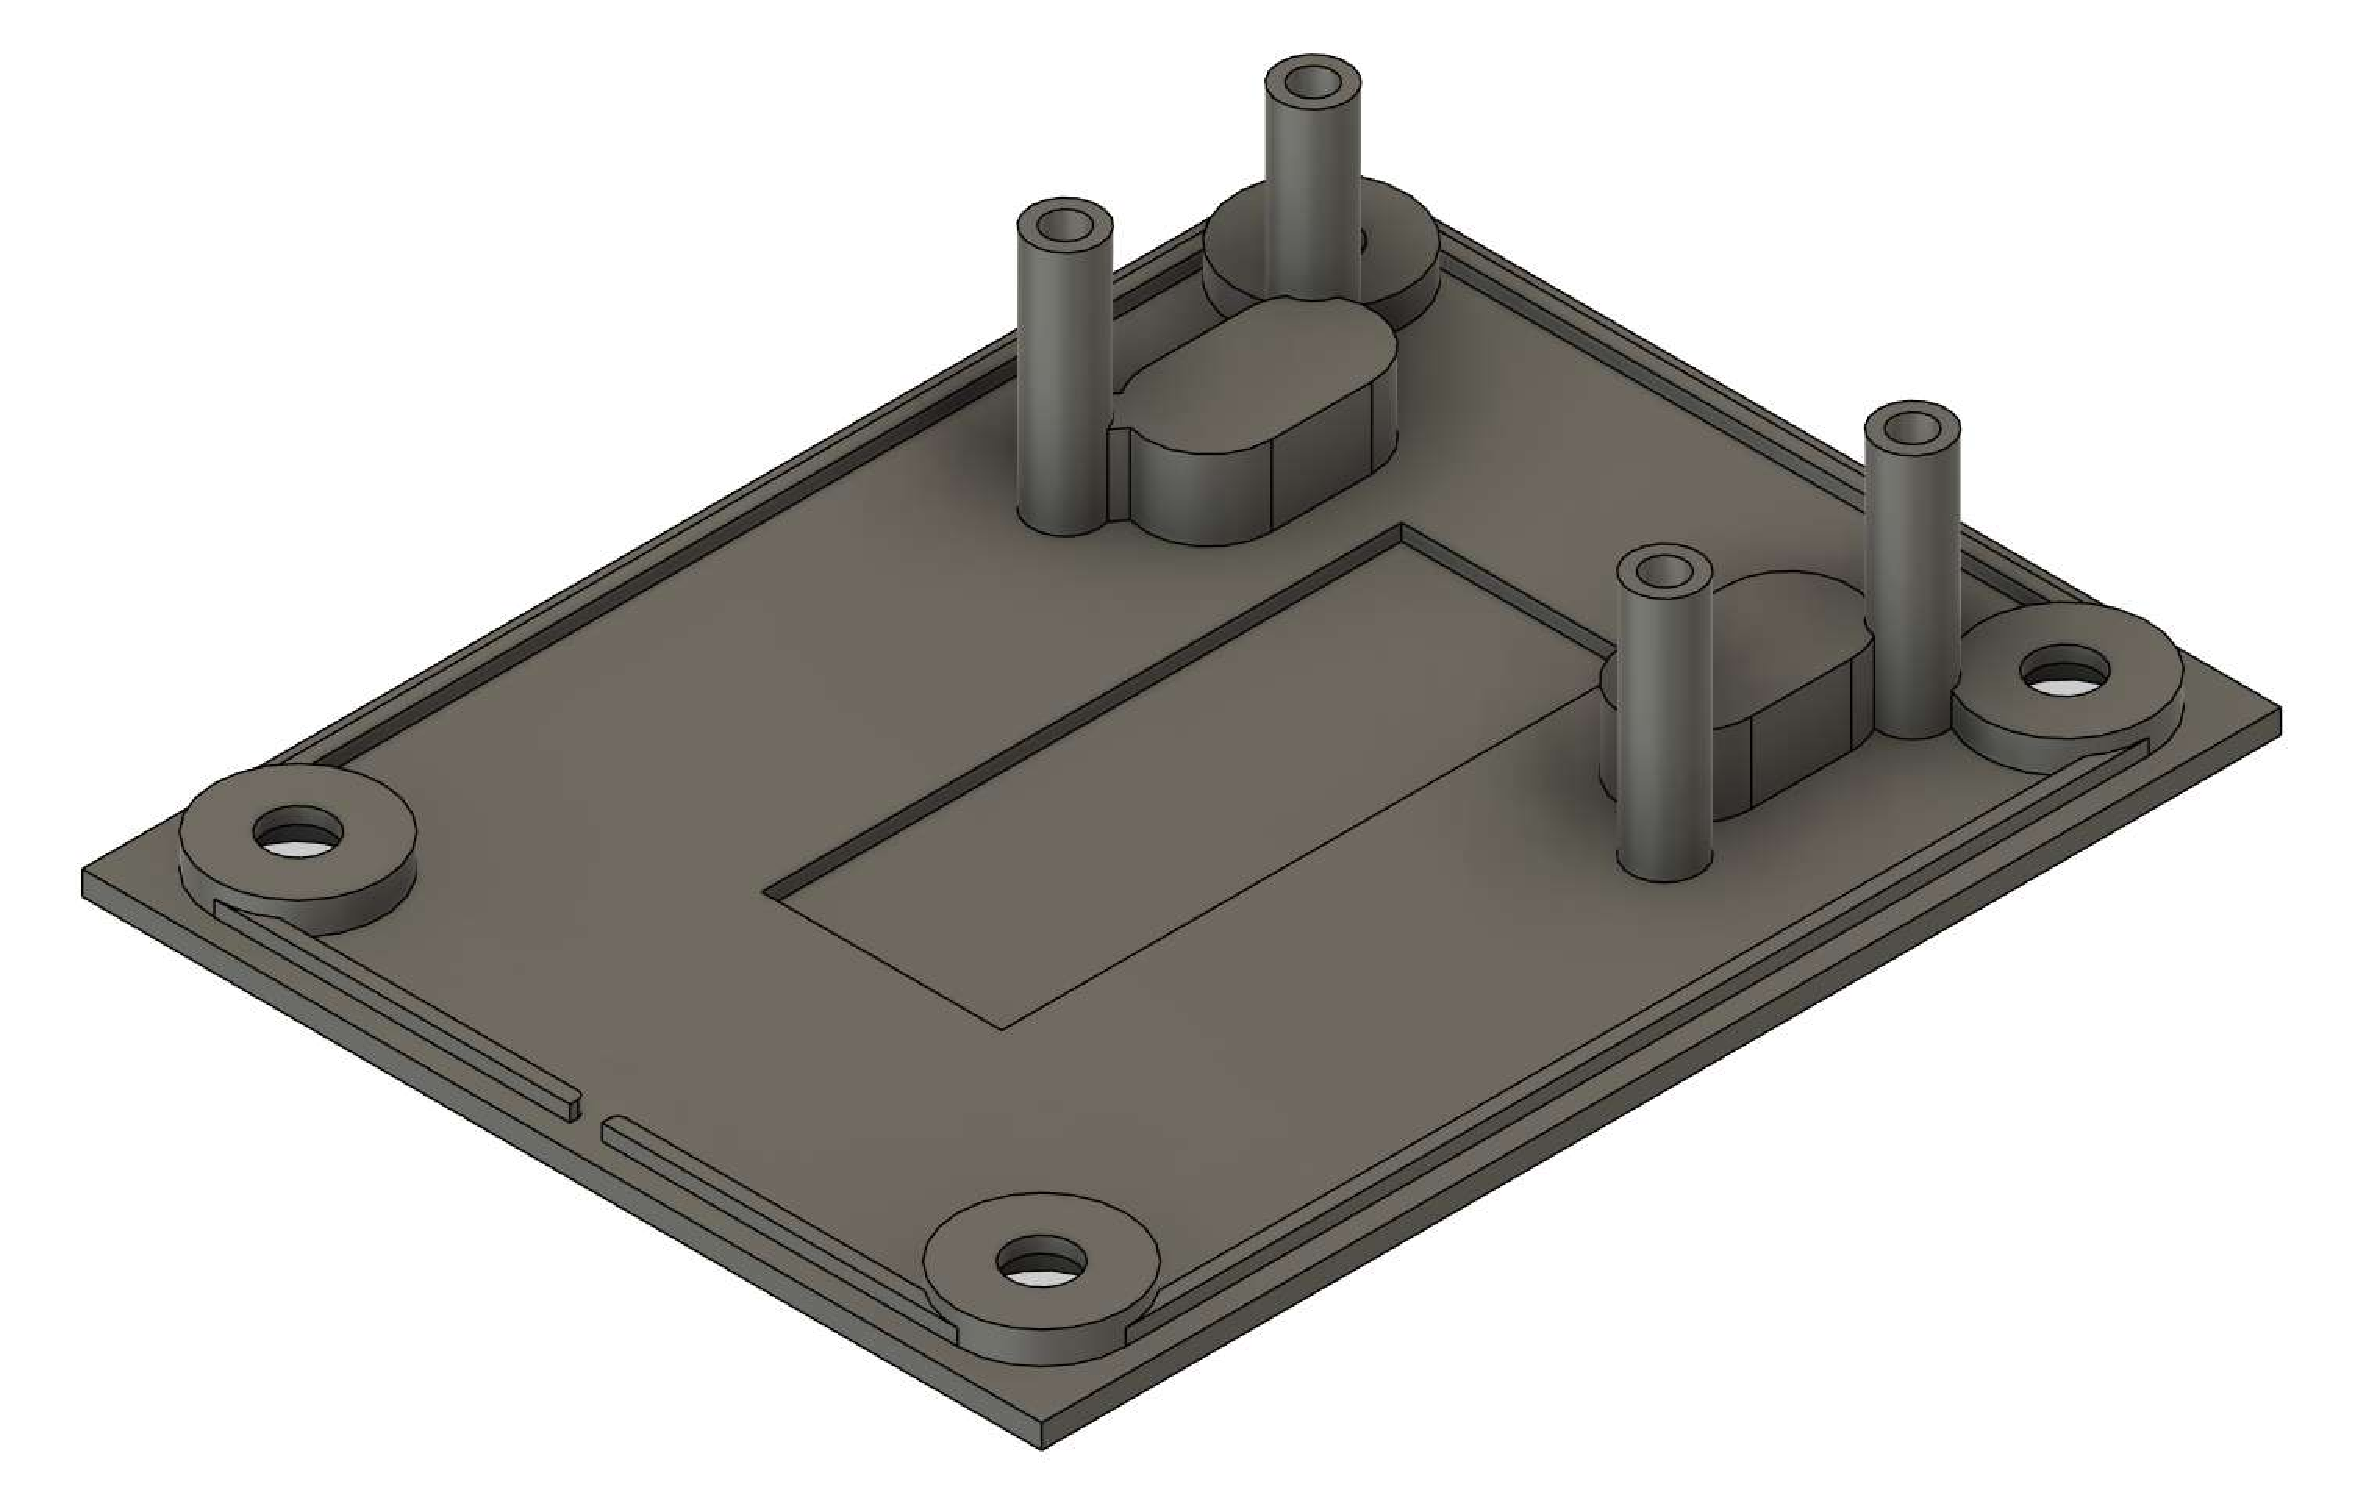
\includegraphics[width=1\textwidth]{Imagenes/Vectorial/backplate_front.pdf}
        \caption{Front side of the enclosure's backplate}
        \label{fig:backplate_front}
    \end{minipage}
    \hfill
    \begin{minipage}[b]{0.49\textwidth}
        \centering
        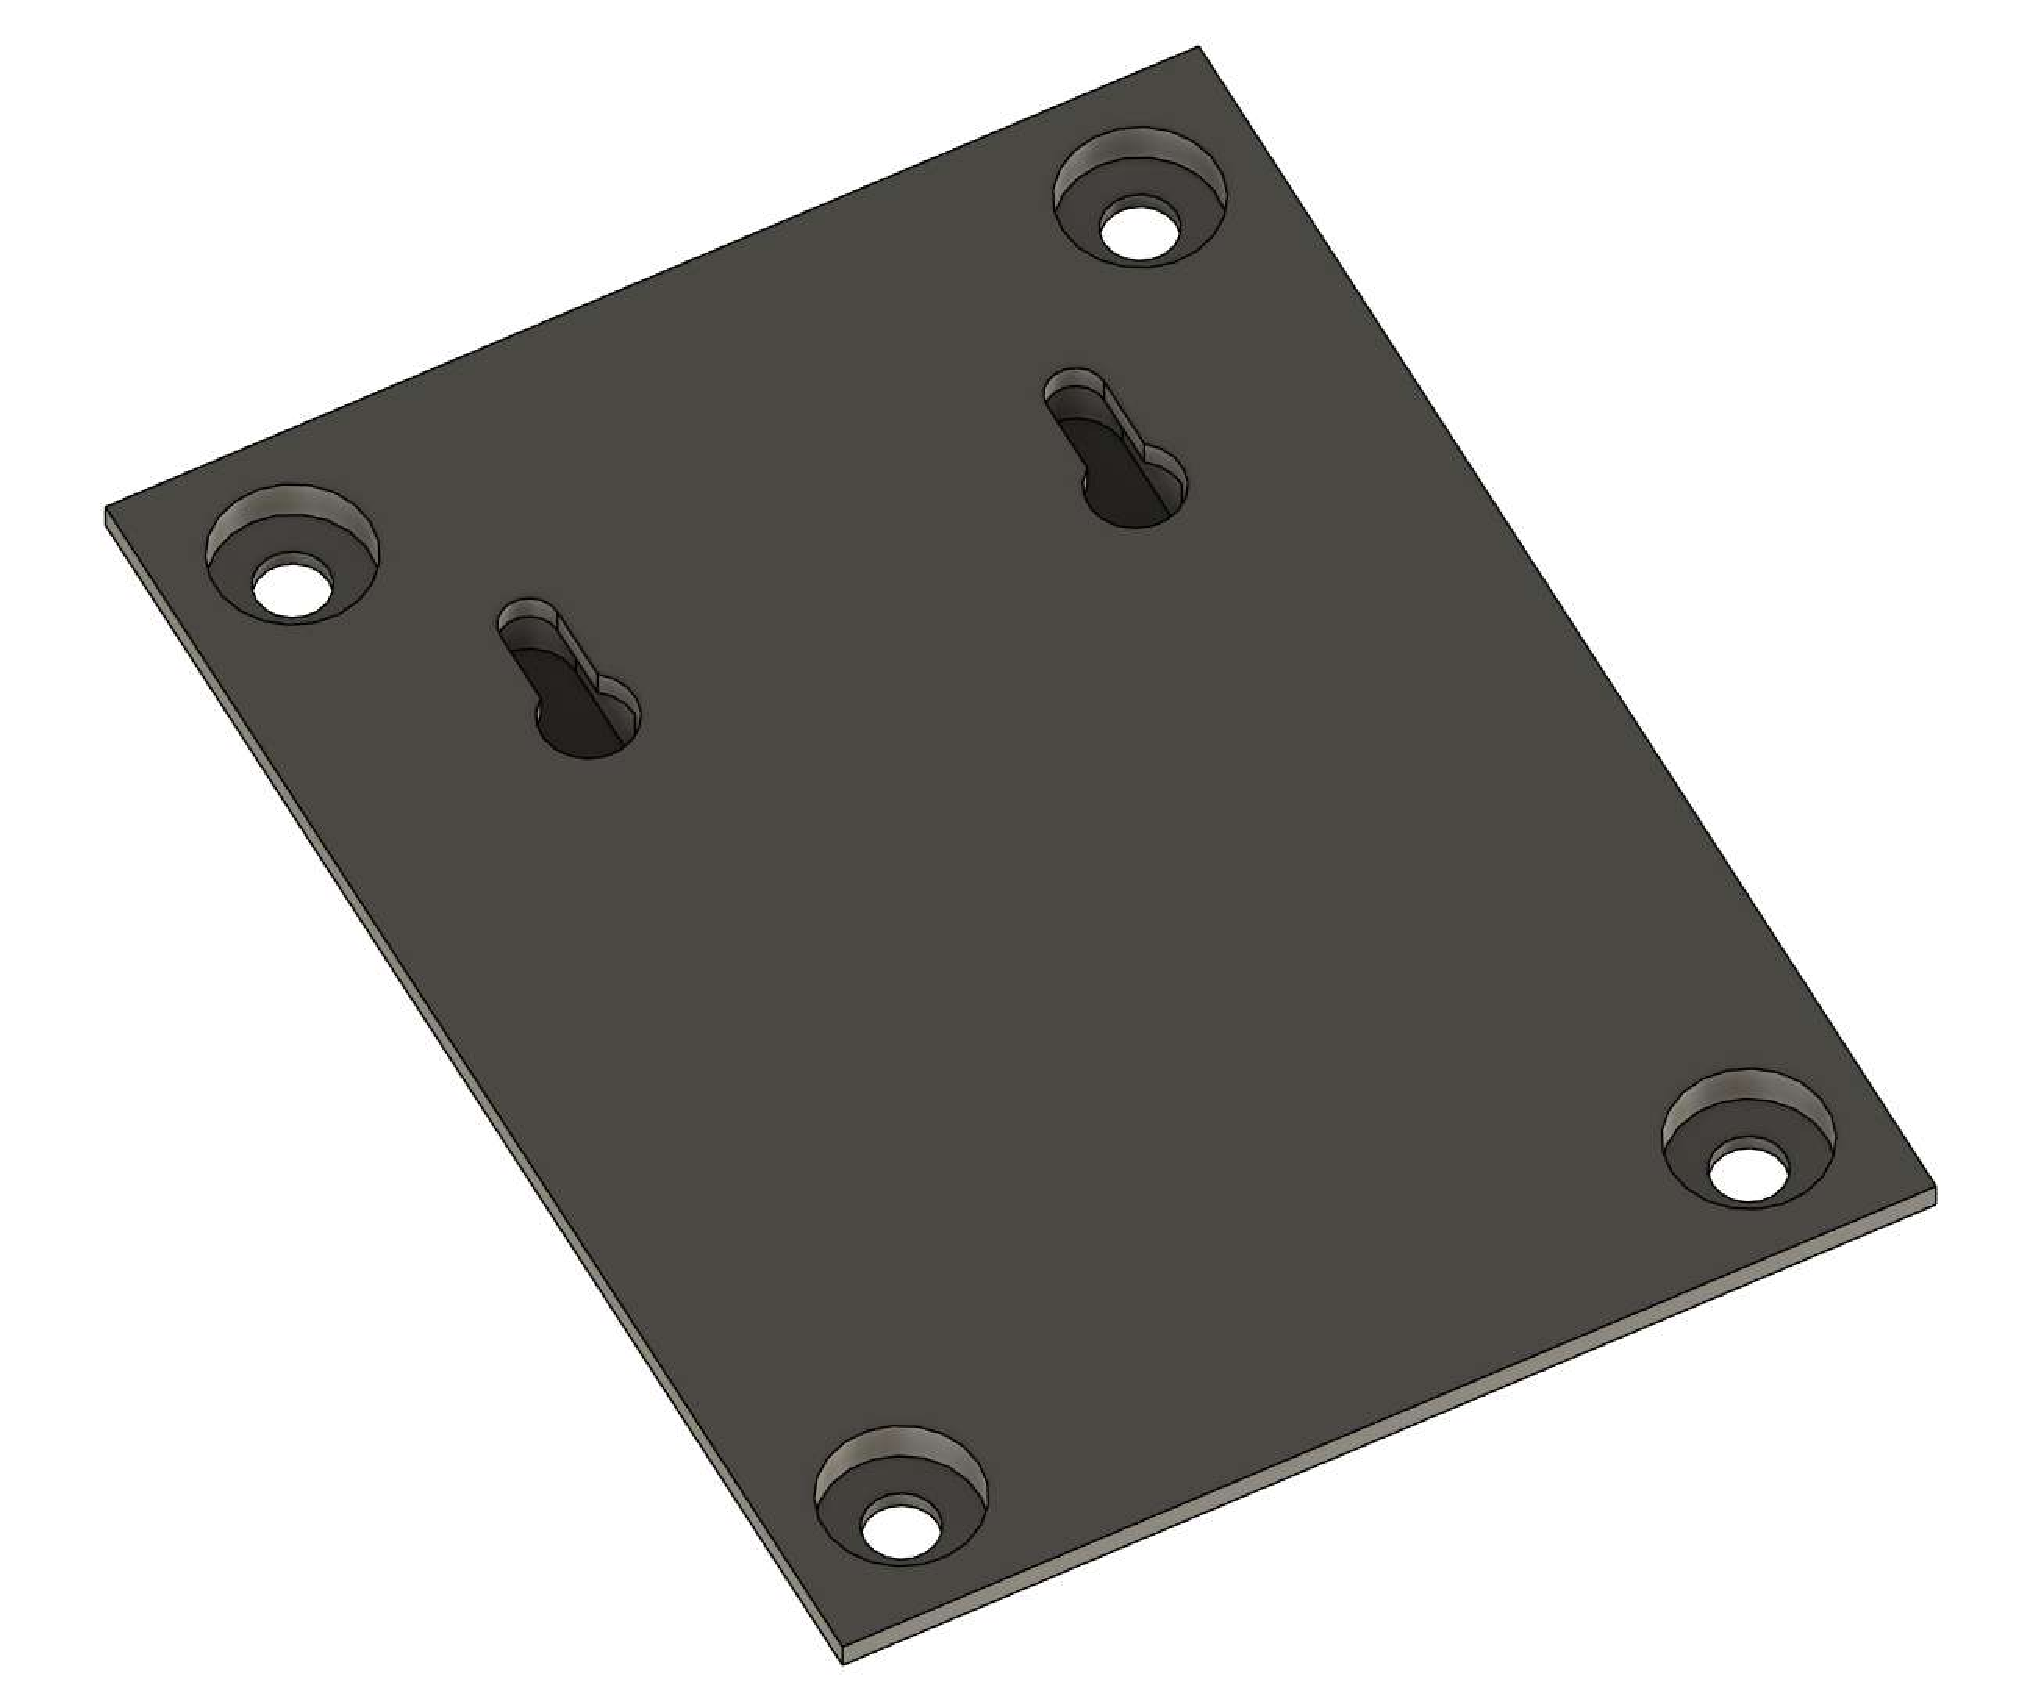
\includegraphics[width=1\textwidth]{Imagenes/Vectorial/backplate_back.pdf}
        \caption{Rear side of the enclosure's backplate}
        \label{fig:backplate_back}
    \end{minipage}
\end{figure}

Another challenging aspect of the design was the mounting mechanism for attaching the backplate to 
the enclosure. Ultimately, it was decided that both parts would be secured together using screws, 
which would be modeled and 3D printed for simplicity. This design required incorporating a 
threaded section on the enclosure side to tighten the screws.

Additionally, there is a recess surrounding the screw holes on the backplate. This recess 
accommodates the screw heads, ensuring they fit flush within the backplate and do not protrude, 
which allows for flat mounting to a wall.

Another important feature of the backplate is the perimeter that protrudes along its edge, as can 
be seen in Figure \ref{fig:backplate_front}. This perimeter holds the backplate laterally, so the 
screws only need to keep the backplate and the enclosure together, without bearing any lateral 
forces. This design detail enhances the structural integrity and durability of the assembled 
enclosure. Moreover, mounting holes were added, for the device to be wall-mounted. This detail can 
be seen in Figure \ref{fig:backplate_back}.

\begin{figure}[h]
	\centering
	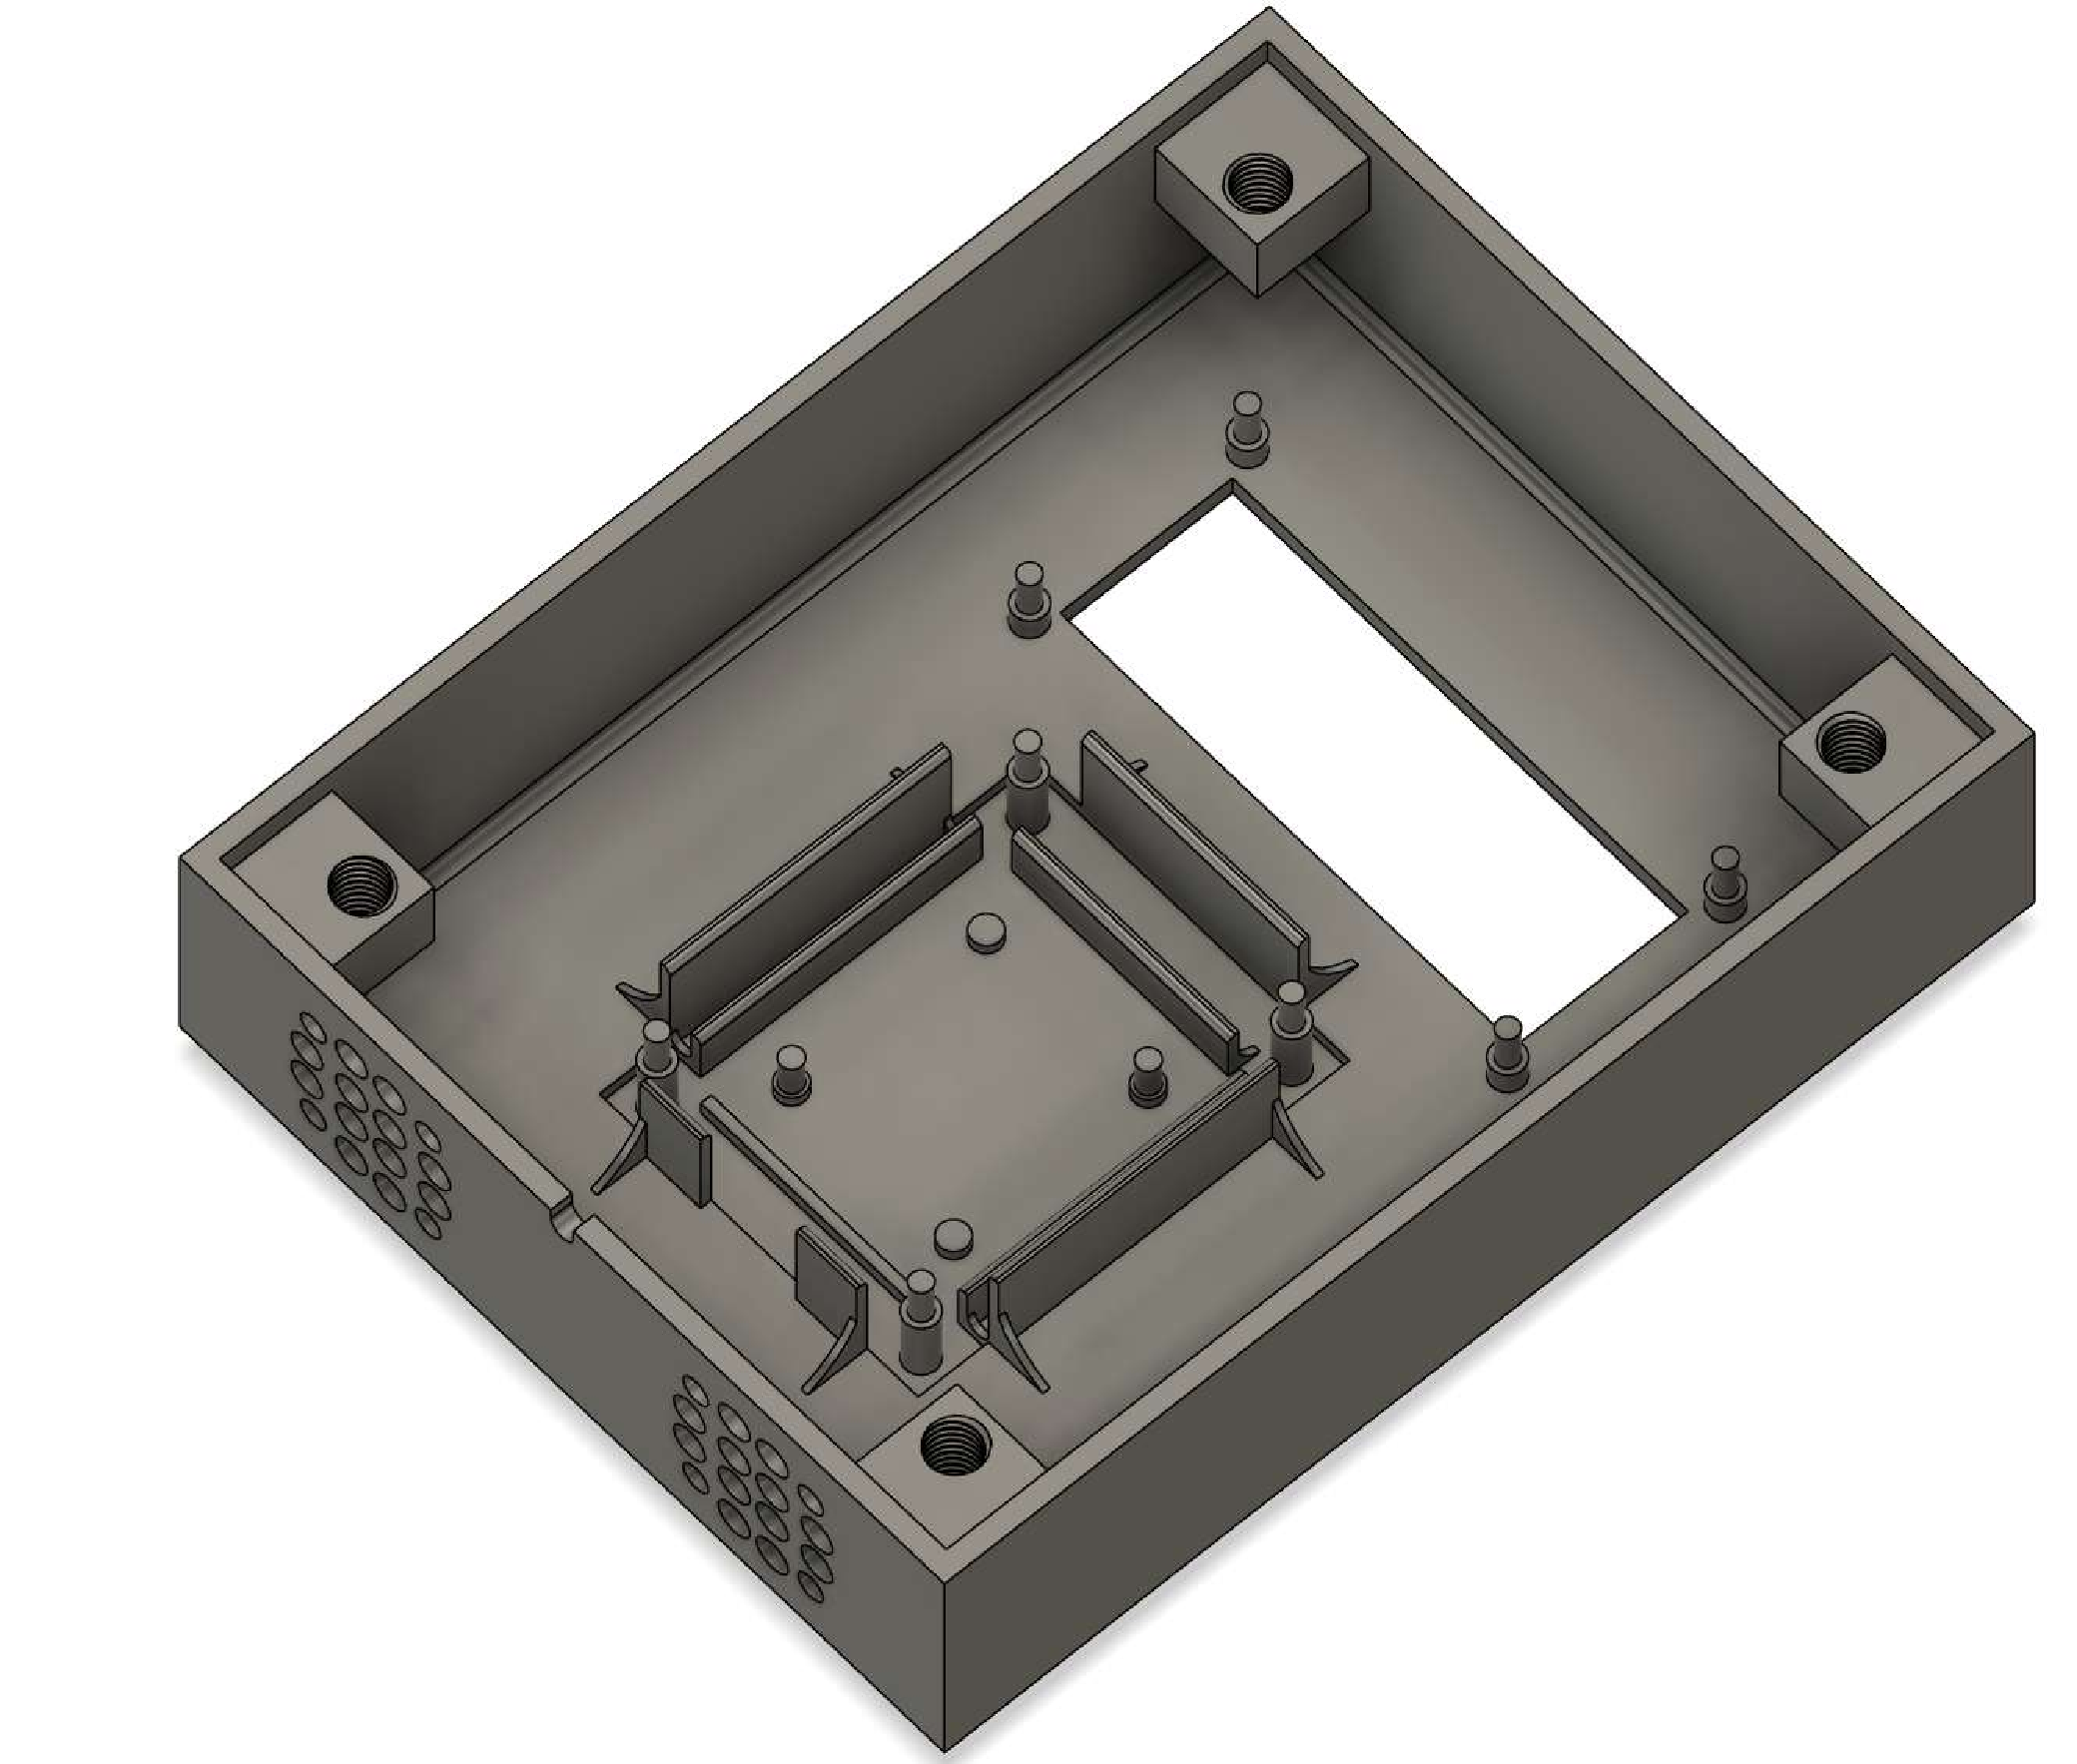
\includegraphics[width = .5\textwidth]{Imagenes/Vectorial/enclosure_back.pdf}
	\caption{Enclosure view from the back}
	\label{fig:enclosure_back}
\end{figure}

Details have already been provided regarding the mounting mechanism for the backplate to the enclosure. Now, the modifications on the enclosure-side will be explored.

A separate component was designed specifically to contain the threads that the screws 
would screw into. These threaded components were then placed in all four corners of the enclosure, 
positioned at the correct distance from the top to ensure the backplate fits flush against them. 
The individual threaded component is illustrated in Figure \ref{fig:enclosure_mounting}, while all 
four components integrated into the enclosure are shown in Figure \ref{fig:enclosure_back}.

\begin{figure}[h]
    \centering
    \begin{minipage}[b]{0.49\textwidth}
        \centering
        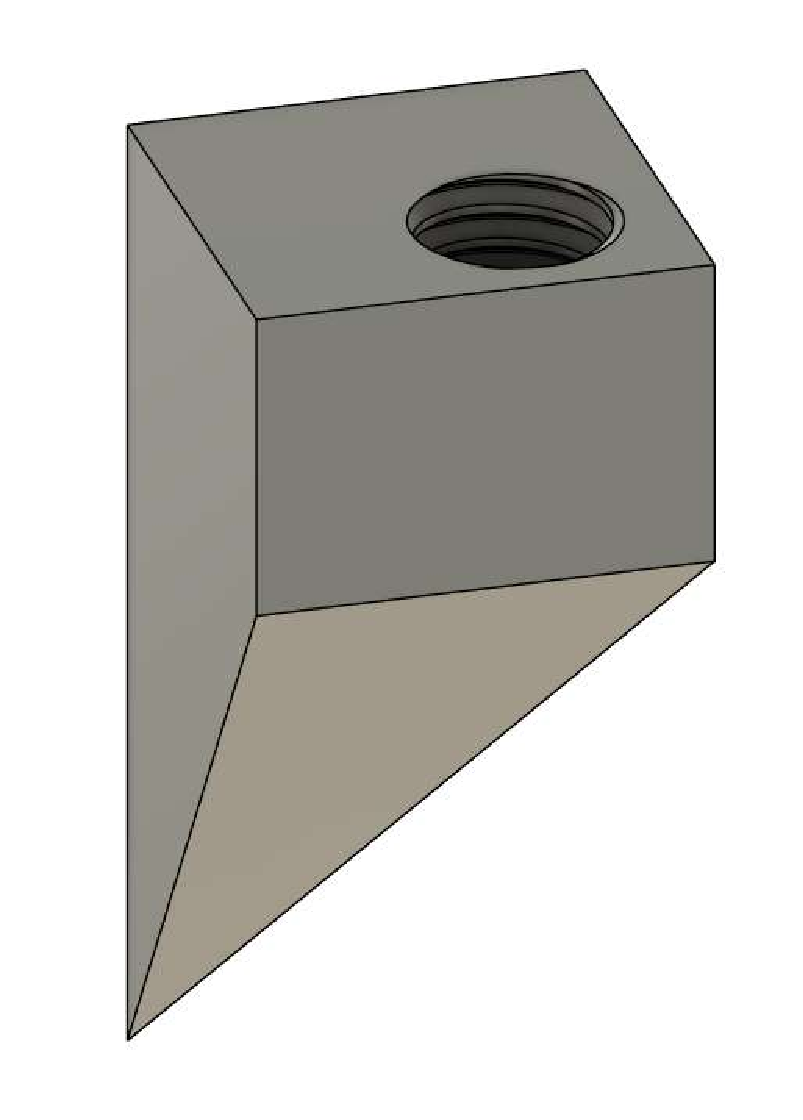
\includegraphics[width=.7\textwidth]{Imagenes/Vectorial/enclosure_mounting.pdf}
        \caption{Enclosure's mounting component}
        \label{fig:enclosure_mounting}
    \end{minipage}
    \hfill
    \begin{minipage}[b]{0.49\textwidth}
        \centering
        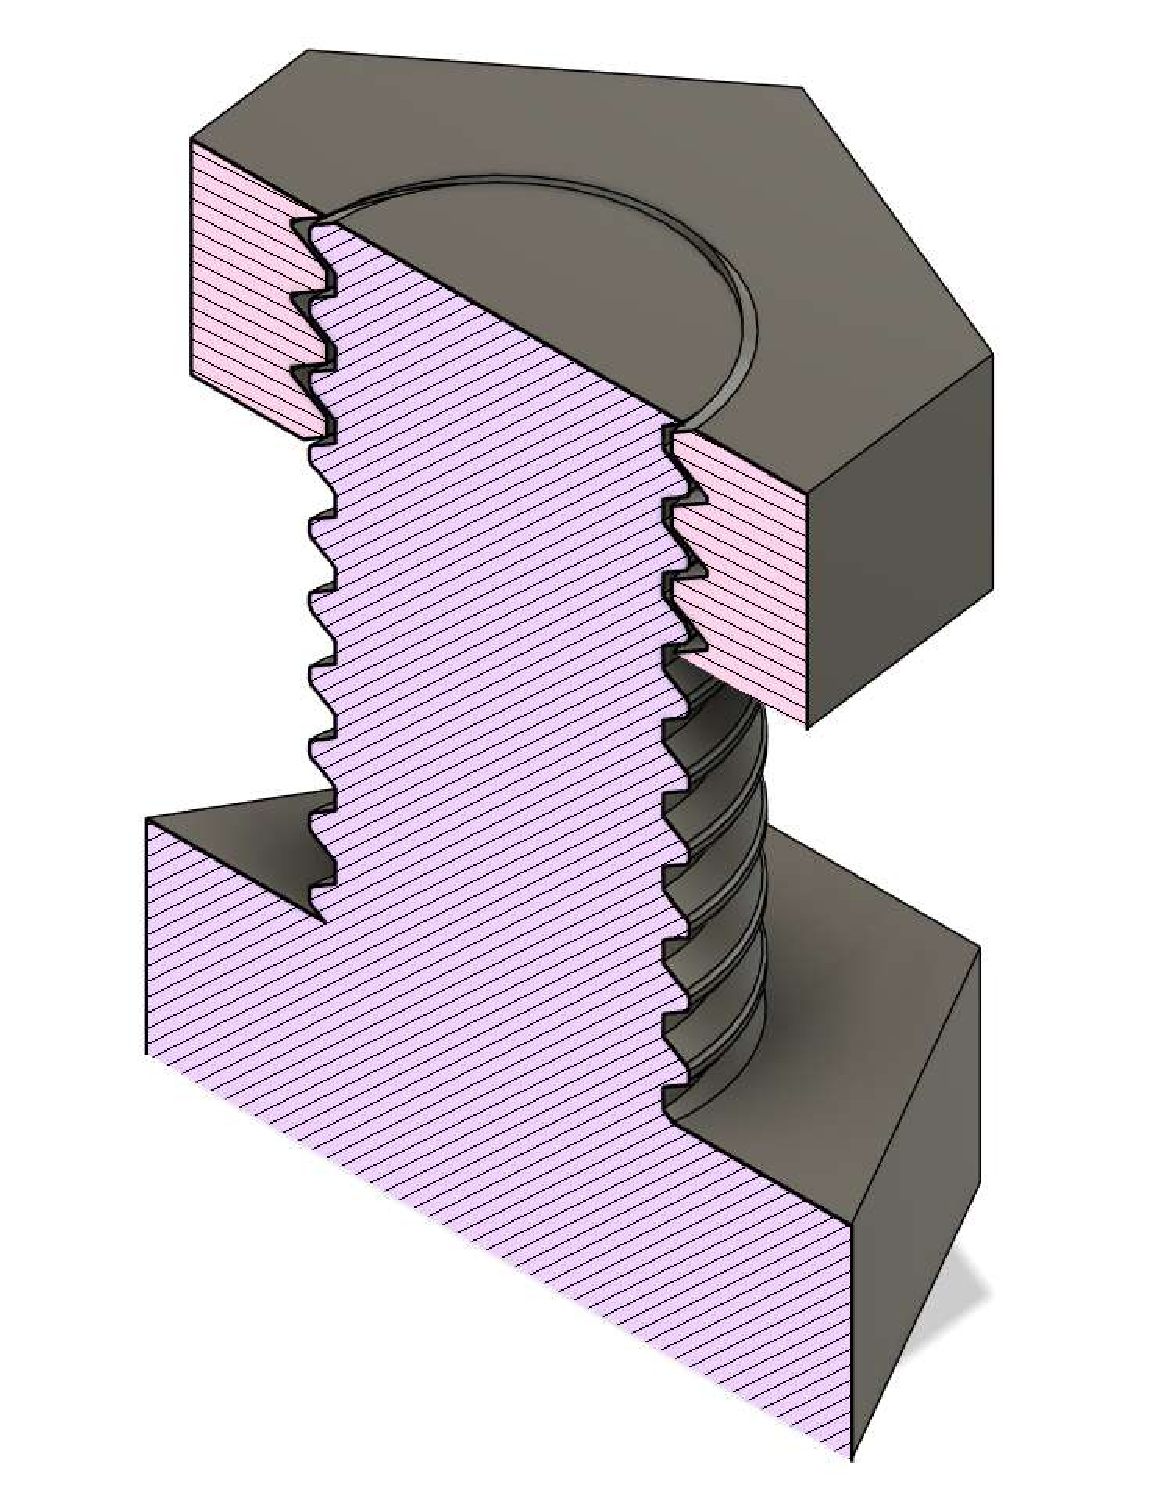
\includegraphics[width=.7\textwidth]{Imagenes/Vectorial/screw_cross_section.pdf}
        \caption{Screw's cross section}
        \label{fig:screw_cross_section}
    \end{minipage}
\end{figure}

Additionally, the screws were 3D printed and modeled using the threading tool in Fusion 360. This 
tool facilitated the creation of an M8 threaded screw, with a diameter of 8 millimeters. To ensure 
functionality, the screw was tested with a nut to verify that it could be smoothly screwed in and 
reused. The cross-section of the screw and nut assembly is illustrated in Figure 
\ref{fig:screw_cross_section}.

The final design details include ventilation holes at the bottom of the enclosure and a slot for 
cable routing. The ventilation holes are intended to allow air circulation, particularly if the 
enclosure is exposed to direct sunlight, to prevent heat buildup. The slot provides a pathway for 
the power cable. Both features are illustrated in Figure \ref{fig:enclosure_back}.


\section{3D Printing}

\subsection{Choosing a 3D Printer}

\subsection{Materials}

\subsection{Printing}
